\documentclass{beamer}

% --- Temi e Colori ---
\usetheme{Madrid}
\usecolortheme{spruce}

\usepackage[utf8]{inputenc}
\usepackage[T1]{fontenc}
\usepackage{graphicx}
\usepackage{xcolor}
\usepackage{caption} % NECESSARIO per \captionof

% Definizione colore personalizzato
\definecolor{darkgreen}{RGB}{0,102,51}
\setbeamercolor{structure}{fg=darkgreen}

% --- Configurazione Link ---
\hypersetup{
    colorlinks=true,
    linkcolor=blue,
    urlcolor=blue
}

% Mostra solo il numero di pagina nel footer
\setbeamertemplate{footline}[page number]

% --- Informazioni Documento ---
\title{Multidimensional Poverty in Sub-Saharan Africa}
\author{Gruppo F: Bondi, Dal Ben, Michetti, Proietti, Veronese}
\date{\today}

\begin{document}
    
    % --- Titolo ---
    \begin{frame}
        \titlepage
    \end{frame}
    
    % --- Research Question ---
    \begin{frame}{Research Question}
        La crescita economica è sufficiente per ridurre la povertà multidimensionale oppure sono necessari interventi mirati?
        \vspace{0.5cm}
        \begin{itemize}
            \item \textbf{Dataset utilizzato:} \href{https://ourworldindata.org/grapher/multidimensional-poverty-index-mpi-hot}{Our World in Data}
        \end{itemize}
    \end{frame}
    
    % --- Domande Descrittive ---
    \begin{frame}{Domande descrittive}
        \begin{itemize}
            \item Evoluzione della povertà multidimensionale (2013--2021)
            \item Confronto tra Senegal, Ghana e Nigeria
            \item Quali fattori della multidimensionalità incidono di più? (MPI)
        \end{itemize}
    \end{frame}
    
    % --- Domande Comparative ---
    \begin{frame}{Domande comparative}
        \begin{itemize}
            \item Differenze tra i paesi analizzati
            \item Povertà multidimensionale vs povertà monetaria
            \item Crescita economica $\rightarrow$ riduzione della povertà?
            \item Impatto dell'istruzione sulla povertà
            \item Investire nel capitale umano è efficace?
        \end{itemize}
    \end{frame}
    
    % --- Selezione Paesi ---
    \begin{frame}{Perché questi paesi? (Senegal, Ghana, Nigeria)}
        \begin{itemize}
            \item Diversi livelli di povertà multidimensionale
            \item Differenti strutture economiche e demografiche
            \item Politiche pubbliche eterogenee
            \item Disponibilità di dataset comparabili
        \end{itemize}
    \end{frame}
    
    % --- Problemi Dati ---
    \begin{frame}{Problema dei dati}
        \begin{itemize}
            \item Serie storiche incomplete (anni mancanti nel dataset MPI)
            \item Difficoltà nel confronto temporale diretto
            \item \textbf{Integrazione dati:} \href{https://databank.worldbank.org/source/world-development-indicators}{World Bank}
        \end{itemize}
    \end{frame}
    
    % --- Interpolazione ---
    \begin{frame}{Interpolazione lineare}
        \begin{itemize}
            \item Stima dei valori mancanti tra le osservazioni
            \item Costruzione di serie temporali continue
            \item \textbf{Processo:} Anni mancanti $\rightarrow$ Stima $\rightarrow$ Serie complete
        \end{itemize}
    \end{frame}
    
    % --- Vantaggi Interpolazione ---
    \begin{frame}{Perché interpolare?}
        \begin{itemize}
            \item Migliora la visualizzazione dei trend a lungo termine
            \item Facilita il confronto diretto tra i paesi
            \item Mantiene la dinamica generale senza distorcere i dati reali
        \end{itemize}
    \end{frame}

    % --- Grafico ---
    \begin{frame}{Grafico interpolato}
        \begin{figure}
            \centering
            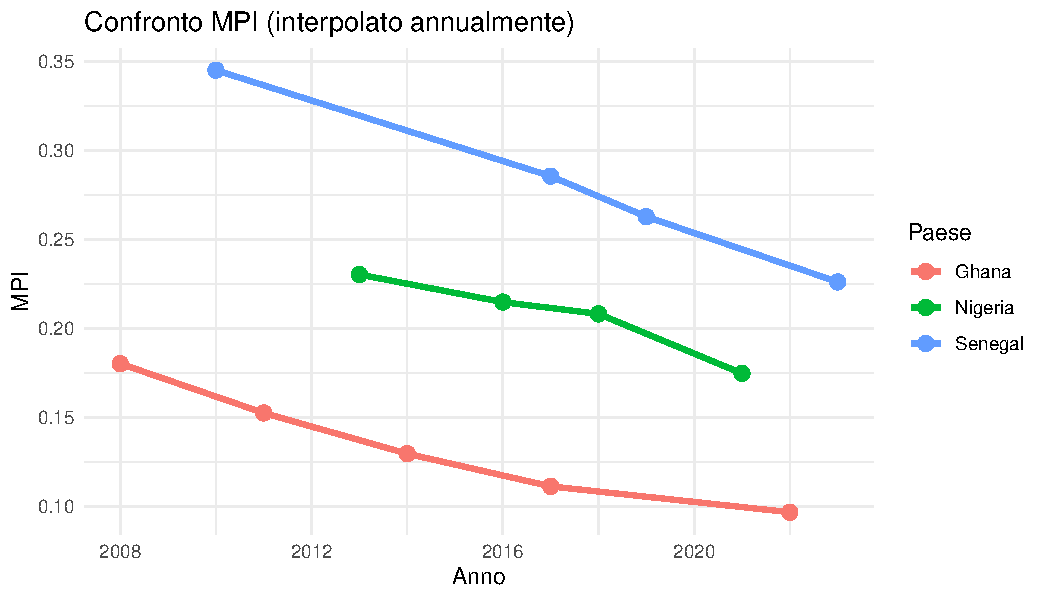
\includegraphics[width=0.75\textwidth]{Grafico1.pdf}
            \caption{Andamento MPI interpolato (2013--2021)}
        \end{figure}
    \end{frame}
    
    % --- Conclusione ---
    \begin{frame}{Conclusione}
        \begin{itemize}
            \item Necessità di un'analisi multidimensionale oltre il PIL
            \item Eterogeneità marcata tra i paesi dell'Africa Subsahariana
            \item Ruolo cruciale delle politiche mirate e dell'istruzione
        \end{itemize}
    \end{frame}
    
    \begin{frame}{Dove eravamo rimasti?}
        \begin{itemize}
            \item Scrivere in modo conciso le domande di ricerca e come vogliamo spiegare l'HDI secondo le variabili.
        \end{itemize}
    \end{frame}
    
    \begin{frame}{Variabili d'interesse:}
        \begin{itemize}
            \item \textbf{FDI (\% PIL)} $\rightarrow$ Investimenti esteri netti
            \item \textbf{Accesso elettricità} $\rightarrow$ \% popolazione con elettricità
            \item \textbf{Acqua potabile} $\rightarrow$ \% popolazione con accesso base
            \item \textbf{Fertilità} $\rightarrow$ Numero medio figli per donna
            \item \textbf{PIL pro capite} $\rightarrow$ Reddito medio per abitante
            \item \textbf{Mortalità} $\rightarrow$ Morti adulti per 1000 (maschile/femminile)
            \item \textbf{Popolazione totale} $\rightarrow$ Numero abitanti
        \end{itemize}
    \end{frame}

    \begin{frame}{HDI nei paesi dell'Africa subsahariana}
        \begin{figure}
            \centering
            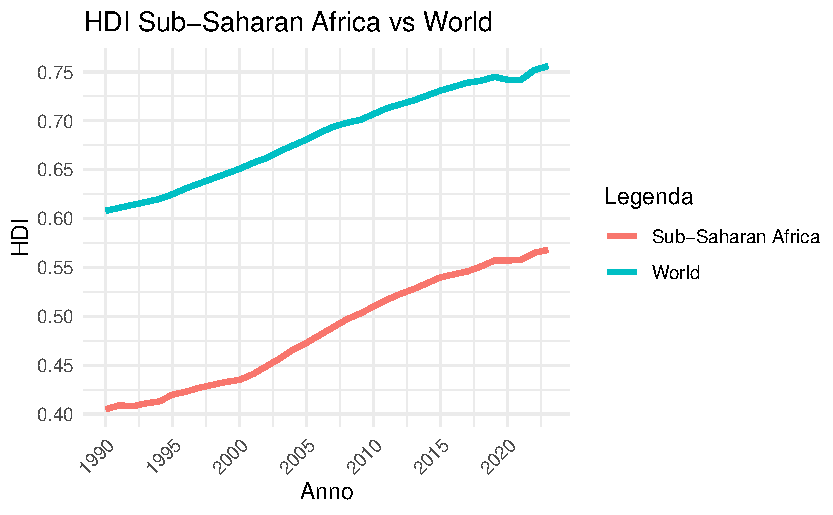
\includegraphics[width=0.7\textwidth]{ggplot2 line chart 1.pdf}
            \caption{Andamento dell'HDI nei paesi in esame}
        \end{figure}
    \end{frame}

    \begin{frame}{GDP per Capita}
        \begin{columns}
            \begin{column}{0.55\textwidth}
                Analisi dei differenti GDP:
                \begin{itemize}
                    \item Sud Africa: GDP più elevato.
                    \item Altri paesi: andamento simile, Nigeria in testa al gruppo.
                \end{itemize}
            \end{column}
            \begin{column}{0.45\textwidth}
                \centering
                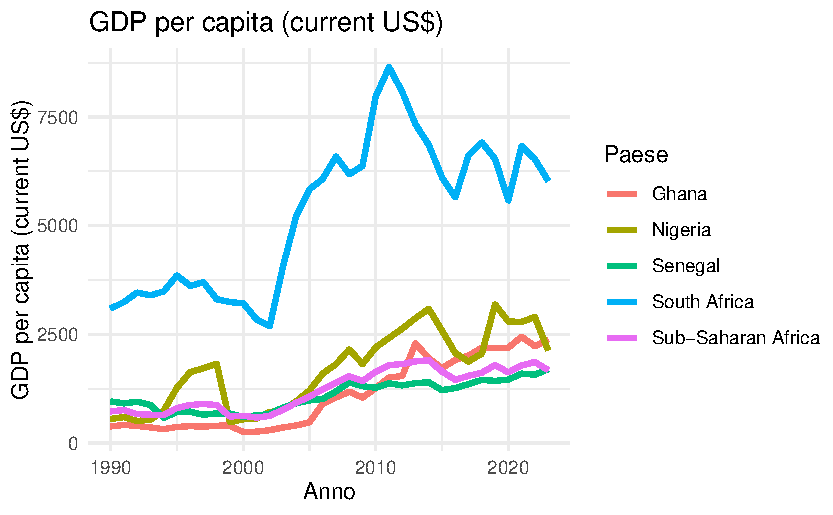
\includegraphics[width=\textwidth]{ggplot2 line chart 3.pdf}
                \captionof{figure}{GDP trend}
            \end{column}
        \end{columns}
    \end{frame}

    \begin{frame}{Acqua ed Elettricità}
        \begin{columns}
            \begin{column}{0.5\textwidth}
                \centering
                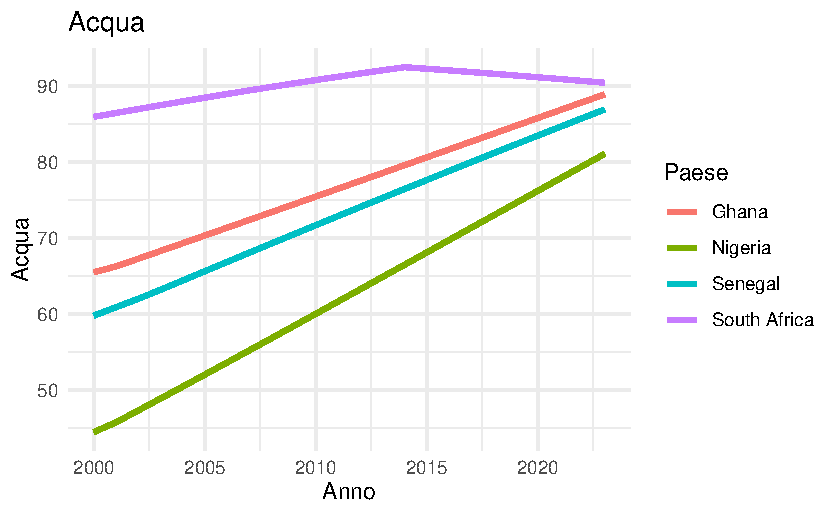
\includegraphics[width=\textwidth]{ggplot2 line chart 5.pdf}
                \captionof{figure}{Trend Acqua}
            \end{column}
            \begin{column}{0.5\textwidth}
                \centering
                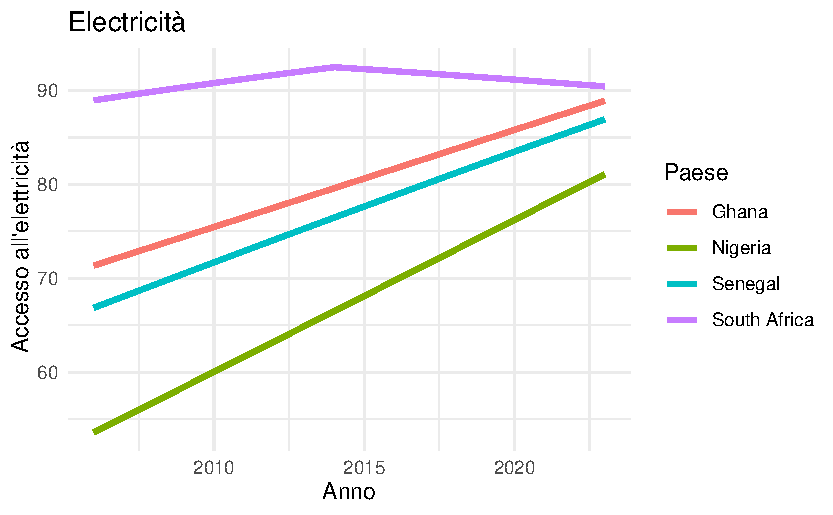
\includegraphics[width=\textwidth]{ggplot2 line chart 8.pdf}
                \captionof{figure}{Trend Elettricità}
            \end{column}
        \end{columns}
    \end{frame}

    \begin{frame}{Analisi Comparativa}
        \begin{columns}[t]
            \begin{column}{0.32\textwidth}
                \centering
                \textbf{\small Fertilità} \\
                \vspace{0.1cm}
                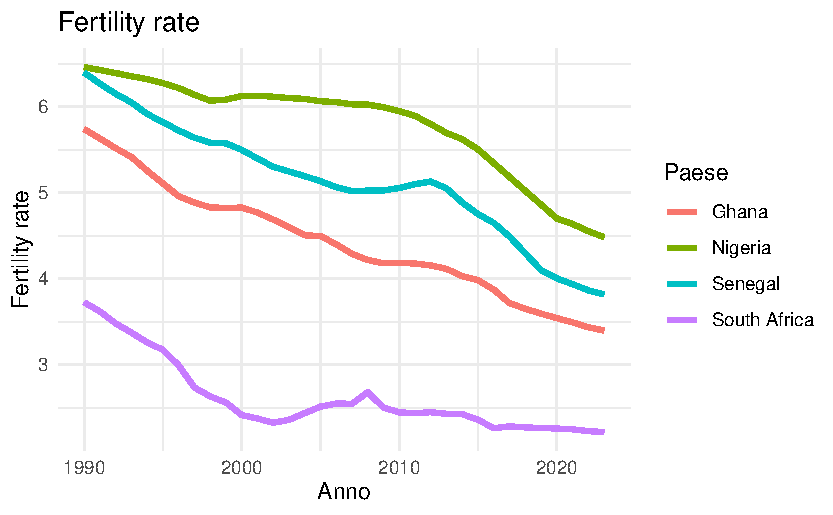
\includegraphics[width=\textwidth]{ggplot2 line chart 4.pdf}
            \end{column}
            \begin{column}{0.32\textwidth}
                \centering
                \textbf{\small Mortalità} \\
                \vspace{0.1cm}
                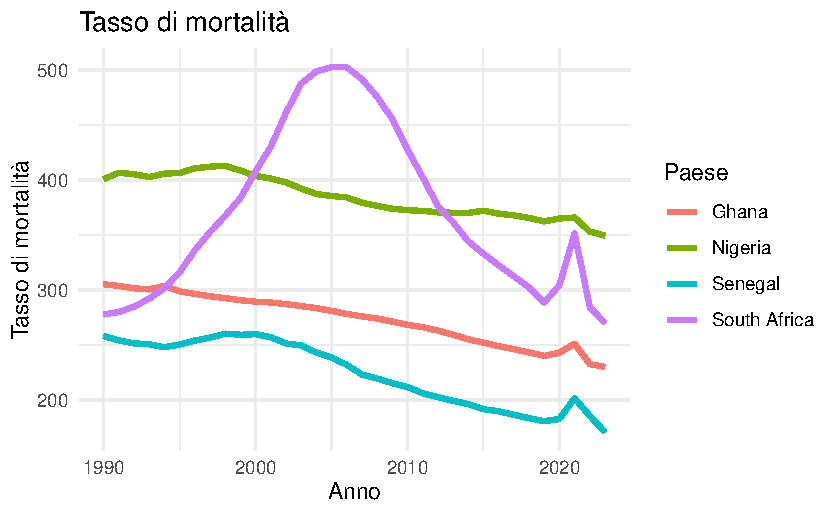
\includegraphics[width=\textwidth]{ggplot2 line chart 6.pdf}
            \end{column}
            \begin{column}{0.32\textwidth}
                \centering
                \textbf{\small Popolazione} \\
                \vspace{0.1cm}
                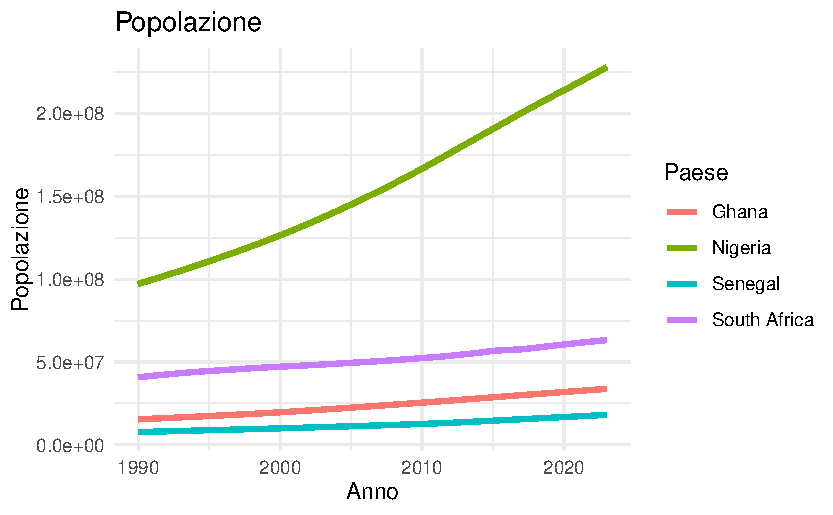
\includegraphics[width=\textwidth]{ggplot2 line chart 7.pdf}
            \end{column}
        \end{columns}
        \vspace{0.4cm}
        \begin{block}{Osservazione}
            \small Pur essendo il primo per GDP, il Sud Africa non domina in tutti gli indicatori (es. popolazione). La ricchezza monetaria non coincide sempre con un migliore tenore di vita multidimensionale.
        \end{block}
    \end{frame}

    \begin{frame}{Investimenti stranieri}
        \begin{columns}
            \begin{column}{0.5\textwidth}
                Investimenti effettuati negli anni:
                \begin{itemize}
                    \item In aumento ovunque tranne che in Ghana.
                    \item Il Senegal mostra una crescita esponenziale recente.
                \end{itemize}
            \end{column}
            \begin{column}{0.5\textwidth}
                \centering
                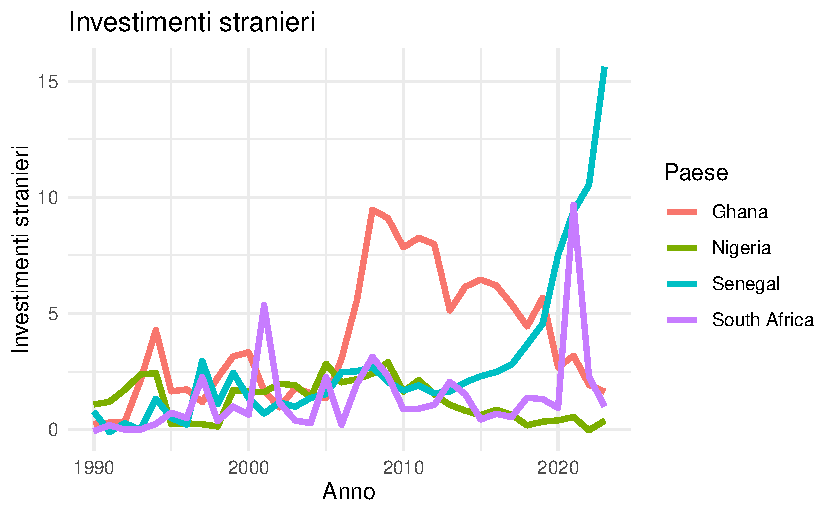
\includegraphics[width=\textwidth]{ggplot2 line chart 9.pdf}
                \captionof{figure}{FDI Trend}
            \end{column}
        \end{columns}
    \end{frame}

\end{document}
